\documentclass[11pt]{article}

\usepackage[a4paper,margin=1in]{geometry}
\usepackage[T1]{fontenc}
\usepackage[utf8]{inputenc}
\usepackage{lmodern}
\usepackage{amsmath,amssymb}
\usepackage{booktabs}
\usepackage{graphicx}
\usepackage{caption}
\usepackage{hyperref}
\usepackage{parskip}
\usepackage{setspace}
\usepackage{lineno}

\setstretch{1.1}

\title{RobustSep: A Stochastic Candidate-Generation Architecture for Robust, Drift-Aware Color Separation}
\author{
  Shreeya Srivastava$^{1,\dagger}$ \and 
  Angad Singh Ahuja$^{1,\dagger}$ \and 
  Pranjal Wala$^{1,\dagger}$ \and 
  Rushabh Lodha$^2$ \\[1.5ex]
  \small $^1$Constrained Image-Synthesis Lab \\
  \small $^2$IIT Mandi
}
\date{}

\begin{document}
\linenumbers

\maketitle
{\def\thefootnote{$\dagger$}\footnotetext{Equal contribution}}

\begin{center}
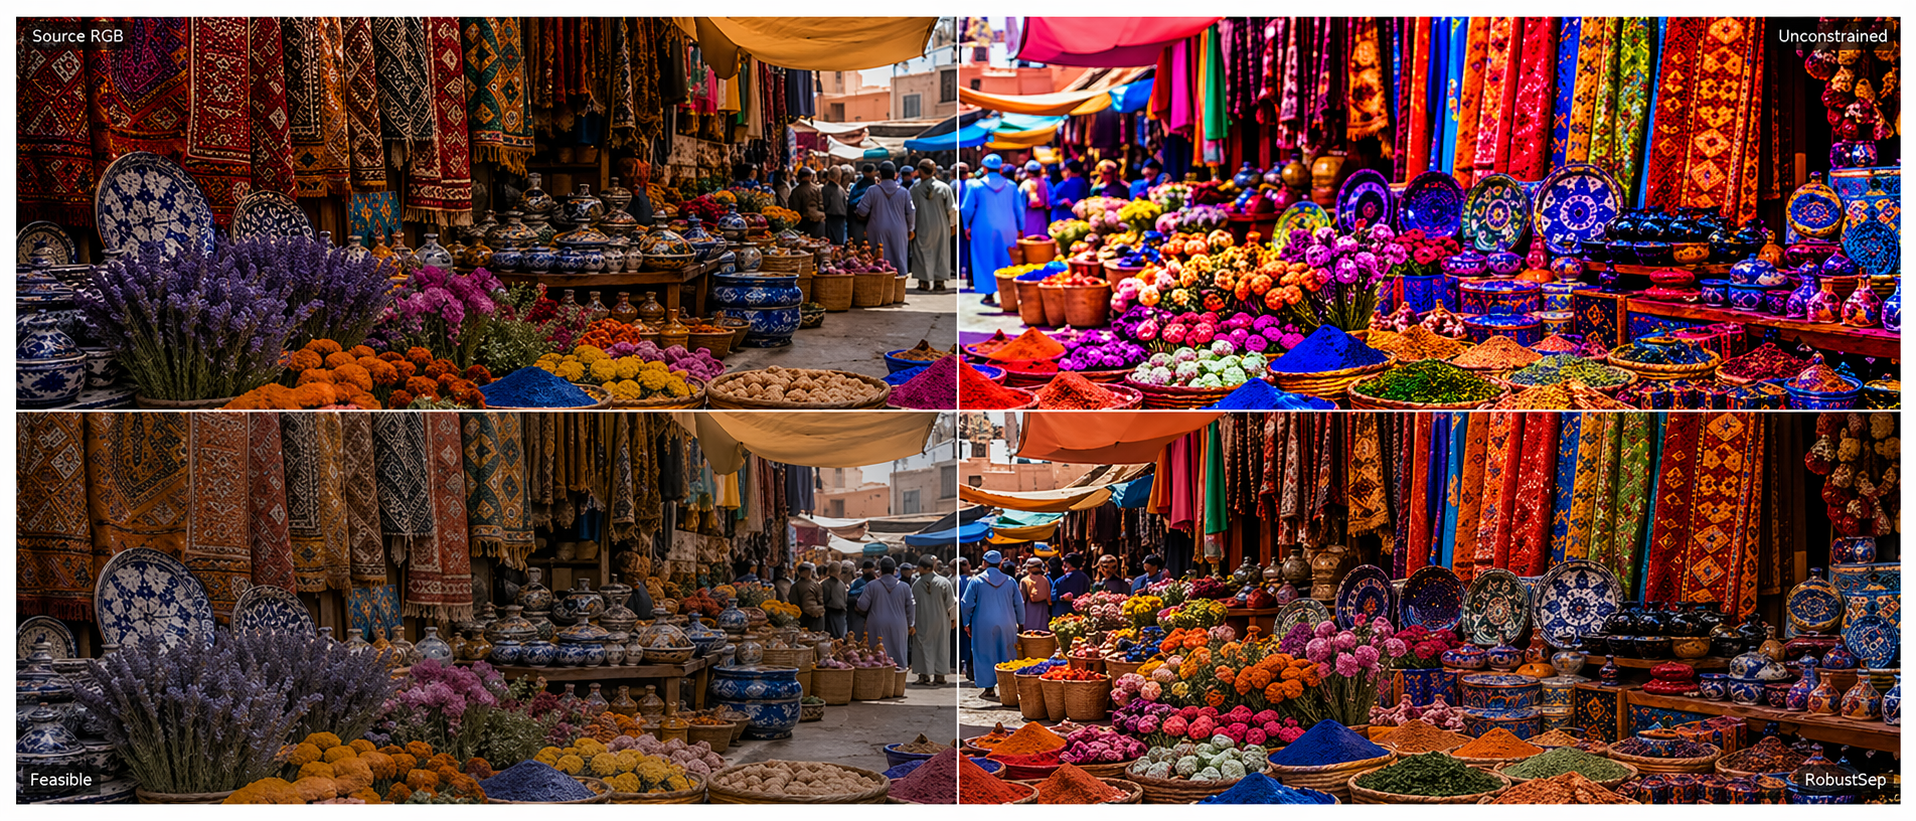
\includegraphics[width=\textwidth]{../figures/robustsep_teaser.png}
\captionof{figure}{Qualitative teaser comparing source RGB appearance with unconstrained, feasibility-projected, and RobustSep separations. The panel illustrates the intended behavior of preserving visual fidelity while enforcing print feasibility and drift-aware robustness.}
\label{fig:teaser}
\end{center}

\begin{abstract}
RGB-to-CMYK color separation for packaging presents a complex inverse problem, characterized by the absence of stable press characterization data and notable physical process drift. Current deterministic approaches, relying on ICC profiles, presuppose idealized conditions and lack formal assurances against perceptual degradation, whereas unconstrained learned models frequently fail to adhere to stringent print-production standards. This paper introduces RobustSep, a stochastic candidate-generation architecture with deterministic replay for packaging color separation that combines stochastic candidate generation, physics-informed refinement, and drift-aware evaluation into a cohesive inference pipeline. At the core of our methodology is the Press Prior Package (PPP), a structured entity encoding process-family constraints and drift distributions, independent of proprietary calibration data. We employ a conditional variational autoencoder (CVAE) for ink candidate generation, which undergoes refinement through a two-pass feasibility pipeline, and is evaluated by a lightweight forward surrogate network under simulated drift conditions. Candidate selection is directed by a 90th-percentile tail-risk criterion across the intent-weighted CIEDE2000 error distribution. Evaluation across five process families is planned; quantitative comparisons against ICC-based and unconstrained learned baselines will be reported once experimental results are obtained. This system establishes a defensible, reproducible framework for semi-automated packaging workflows. Code is available at \url{https://github.com/AngadSingh22/RobustSep.git}.
\end{abstract}

\noindent\textbf{Keywords:} RGB-to-CMYK separation, packaging color management, robust optimization, conditional variational autoencoder, process drift.

\section{Introduction}

Converting RGB images to the CMYK colour space required by physical printing presses is a genuinely ill-posed inverse problem: for any target colour, a continuous family of ink combinations can produce perceptually equivalent printed appearances. Physical ink behaviour on substrate is governed by the nonlinear Neugebauer equations, dot-gain effects, and ink-masking interactions \cite{ulichney,rodriguez}; the resulting system of equations is non-injective and cannot be analytically inverted \cite{ulichney,rodriguez}. A further complication is the black (K) channel ambiguity: any chromatic dark region can be reproduced by combining cyan, magenta, and yellow, or by substituting part of that mixture with black ink through Gray Component Replacement (GCR). Aggressive GCR reduces ink cost and improves press stability but introduces visible halftone granularity in smooth tonal areas, an effect particularly objectionable in skin tones and brand flat-tints. Any practical separation algorithm must therefore balance perceptual fidelity, ink economy, hard physical limits such as Total Area Coverage (TAC), and stability across the mechanical variability inherent to real presses.

The foundational treatment of RGB-to-CMYK conversion in print production was formalised by Rodriguez \cite{rodriguez}, whose graphic arts pipeline remains the implicit industry reference. The pipeline proceeds in three stages: a direct channel inversion establishes the baseline
\[
C = 1 - R, \qquad M = 1 - G, \qquad Y = 1 - B;
\]
hue-family corrections apply channel-specific additive offsets of the form
\[
C' = C + \alpha_h,
\]
where $\alpha_h$ is a scalar calibrated per hue family to compensate for spectral impurities in real-world inks, applied across six dominant hue regions; and a parametrised tone curve of the form
\[
K = f\bigl(\min(C,M,Y)\bigr)
\]
controls black generation, where $f$ is a piecewise-linear function defining the K channel's activation threshold, rise slope, and upper limit. Evaluation within this paradigm is perceptual: neutral tone reproduction, hue accuracy across the six families, transition smoothness at colour-family boundaries, and tone reproduction curve fidelity constitute the minimum threshold for a commercially viable separation. These criteria remain foundational for all subsequent methods. The pipeline's principal limitation is that all correction parameters are assumed rather than measured from actual press response; any deviation of real ink spectral behaviour from the assumed model propagates uncorrected into the separation, with no mechanism for quantifying or bounding the resulting perceptual error.

\section{Related Work}

The heuristic graphic arts pipeline operates on assumed ink behaviour rather than measured press response. Zeng \cite{zeng} addressed this directly by proposing a five-stage deterministic framework for constructing three-dimensional look-up tables (LUTs) from direct colorimetric press measurement. The process prints and measures a structured CMYK patch set, fits per-channel one-dimensional tone curves to the measured densities, builds a 3D LUT populating nodes outward from the neutral axis, and applies GCR and Under Colour Removal (UCR) rules with localised K-control. By grounding the LUT in measured rather than assumed ink behaviour, Zeng's framework achieves significantly larger gamut volumes in high-chroma shadow regions, while enforcing hard TAC constraints at every LUT node. The key contribution is the introduction of gamut volume in CIE Lab space as an explicit optimisation target, a criterion that all subsequent data-driven methods inherit. However, even with TAC and gamut constraints satisfied, the framework offers no model of press variability: the LUT encodes a single static press state, provides no mechanism for bounding perceptual error when ink viscosity, temperature, or substrate absorption drifts from the characterisation conditions, and must be fully rebuilt whenever process conditions change materially.

The memory footprint of high-resolution 3D LUTs (approximately 32 MB for an 8-bit LUT) motivated early use of neural networks as compact approximators. Marcu and Iwata \cite{marcu} trained a 3-12-12-12-4 multilayer perceptron on synthetic CMYK to RGB forward mappings computed via the Neugebauer equations with Yule-Nielsen corrections, demonstrating that a learned model could approximate the highly nonlinear inverse mapping. In parallel, the ICC profile specification standardized the architecture and data representation used by device color-management workflows \cite{icc}. These approaches confirmed the viability of compact data-driven and profile-based colour-space inversion, but shared a limitation: the resulting mappings encoded a globally fixed GCR policy, with no sensitivity to the spatial frequency, tonal character, or semantic content of specific image regions.

Chen et al.\ \cite{chen} introduced the first spatially heterogeneous formulation of RGB-to-CMYK separation, treating it as a multi-objective deterministic optimisation problem rather than a global mapping. Their framework computes a weighted local entropy over a $9\times 9$ pixel window, reducing raw Shannon entropy by the local standard deviation to avoid false positives in uniform regions to produce an Activity Level (AL) map. A semantic skin-detection protocol in LCH space generates an Activity Level Multiplier (ALM); the two are fused via a Guided Filter to produce the final Activity Map (AM). The AM establishes a per-pixel ceiling $K_{\text{target}}$ for black ink generation. The optimisation then minimises total CMYK channel sum (reducing TAC) while maximising K substitution without exceeding $K_{\text{target}}$:
\[
\text{minimise } \sum (C + M + Y + K)
\quad \text{subject to} \quad
K \leq K_{\text{target}}, \qquad \sum (C + M + Y + K) \leq TAC_{\max}.
\]
This approach achieved 10--25\% verifiable ink savings with 67--90\% of pixels held below $\Delta E_2 = 3$. The critical unresolved limitation, however, is the assumption of a perfectly stable press: the framework characterises and optimises for a single nominal press state and provides no mechanism for evaluating or bounding perceptual deviation under process drift.

Bo and Cao \cite{bo} introduced ColorNet, the most recent purely data-driven approach prior to this work. ColorNet maps RGB inputs into a 1024-dimensional feature space via fully connected layers with batch normalisation and ReLU, applies a channel attention mechanism using global average pooling
\[
z = \operatorname{GAP}(X) = \frac{1}{HW}\sum_{i,j} X_{ij}
\]
to reweight per-channel feature importance, processes the recalibrated features through seven residual blocks with DenseNet-style skip connections, and maps to CMYK via a sigmoid output head. Training on two million Gaussian-augmented RGB-CMYK pairs across five ICC profiles, with CIE Lab as an intermediate perceptual space, ColorNet achieved a mean $\Delta E_{00}$ of 0.2554 under the Japan Color 2001 Coated profile against Photoshop's 0.8157. Despite this strong nominal performance, ColorNet is a deterministic, single-estimate model with no constraint enforcement, no GCR policy control, and no mechanism for robustness evaluation under press drift. This limitation reflects a broader gap: the ability of learned systems to match or exceed classical pipelines on average perceptual accuracy does not by itself confer deployability under the hard constraints and process variability of production print. Specifically, ColorNet cannot generalise across press families without full retraining on that family's ICC profiles; it provides no mechanism for specifying or enforcing ink limits such as TAC or per-channel caps; it produces a single separation with no indication of whether that separation will remain acceptable under the process variation that occurs within a normal production run; and it offers no fallback or escalation policy when a proposed separation is physically inadmissible.

The collective progression from Rodriguez \cite{rodriguez} to ColorNet \cite{bo} traces a clear arc: from heuristic inversion to empirically grounded LUTs, then to learned global approximators, then to spatially adaptive optimisation, and finally to deep attention-guided networks. Each generation addressed the limitations of its predecessor. Rodriguez \cite{rodriguez} assumes ink spectral behaviour rather than measuring it, with no mechanism for bounding error when real inks deviate from the assumed model. Zeng \cite{zeng}, despite grounding separation in measured press data and enforcing hard TAC constraints, encodes a single static press state that must be rebuilt entirely whenever process conditions change. Compact neural approximators such as Marcu and Iwata \cite{marcu} confirm the viability of learned inversion but encode a globally fixed GCR policy with no spatial or semantic sensitivity. Chen et al.\ \cite{chen} introduce spatial adaptivity but optimise for a single nominal press state, with no mechanism for evaluating perceptual deviation under process variation. ColorNet \cite{bo}, despite strong nominal accuracy, cannot generalise across press families without retraining, enforces no physical printability constraints, and provides no robustness evaluation under drift. Taken together, every prior method shares two structural gaps that none has resolved simultaneously: the universal assumption of a stable, fully characterised press with no formal model of process drift; and a single, deterministic separation output that discards the solution diversity inherent to the underdetermined inverse problem. These gaps reflect a sustained absence of robustness-first thinking in a domain where production press conditions vary continuously and the cost of a failed run is substantial. RobustSep is introduced to address both gaps within a single architecture, combining inference-time process priors, stochastic candidate generation, physics-informed feasibility enforcement, and drift-aware candidate selection.

\section{Methodology}

\subsection{Problem Formulation}

RGB-to-CMYK color separation is an underdetermined inverse problem meaning that multiple ink configurations can produce perceptually equivalent appearances for a given RGB input. Rather than committing to a single deterministic mapping, we pose separation as a constrained optimization problem that explicitly accounts for printability and process variability.

Given an RGB patch $x_u$, the objective is to recover an ink separation $y_u$ that lies within a feasible set defined by a Press Prior Package (PPP). RobustSep uses CMYKOGV as its canonical internal separation space, where $O$, $G$, and $V$ denote expanded-gamut Orange, Green, and Violet inks; downstream CMYK export is treated as a separate documented conversion step when required. This feasible set enforces hard constraints such as per-channel ink limits and a maximum total area coverage (TAC), ensuring that all admissible solutions are physically printable. For the internal channel set $\mathcal{C}=\{C,M,Y,K,O,G,V\}$, a candidate patch $y$ belongs to $K(\mathrm{PPP})$ if every pixel satisfies
\[
0 \leq y_c \leq \kappa_c,\quad
\sum_{c\in\mathcal{C}} y_c \leq TAC_{\max},\quad
y_O+y_G+y_V \leq OGV_{\max},
\]
\[
y_C+y_O \leq \rho_{CO},\qquad
y_M+y_G \leq \rho_{MG},\qquad
y_Y+y_V \leq \rho_{YV},
\]
with the additional neutral/dark constraint
\[
y_O+y_G+y_V \leq OGV_{\mathrm{neutral}}
\quad\text{when}\quad
\sqrt{a^{*2}+b^{*2}} \leq \tau_{\mathrm{chroma}}
\ \text{or}\ 
L^* \leq \tau_{\mathrm{dark}}.
\]
Here $\kappa_c$ are per-channel caps, $\rho_{CO},\rho_{MG},\rho_{YV}$ are expanded-gamut pair caps, and the neutral/dark thresholds are resolved from the PPP.

To account for real-world variability in printing, we evaluate each candidate separation under stochastic perturbations that model changes in tone reproduction and ink behavior. For a given $y_u$, this induces a distribution of perceptual errors with respect to the target appearance. Instead of minimizing average error, we minimize a tail-risk measure, defined as the 90th-percentile perceptual deviation under these perturbations.

The resulting optimization problem can be expressed as
\[
y_u^* = \arg\min_{y_u \in K(\mathrm{PPP})} R_{0.90},
\]
where $K(\mathrm{PPP})$ denotes the set of feasible ink configurations and $R_{0.90}$ captures worst-case perceptual error under PPP-conditioned process drift. We denote by $\Pi_K$ the deterministic projection operator that maps any candidate patch back into this feasible set.

Figure~\ref{fig:system_manifold} summarizes the operator-level pipeline before we detail PPP conditioning, stochastic proposal, feasibility projection, and drift-risk selection.

\begin{figure}[t]
\centering
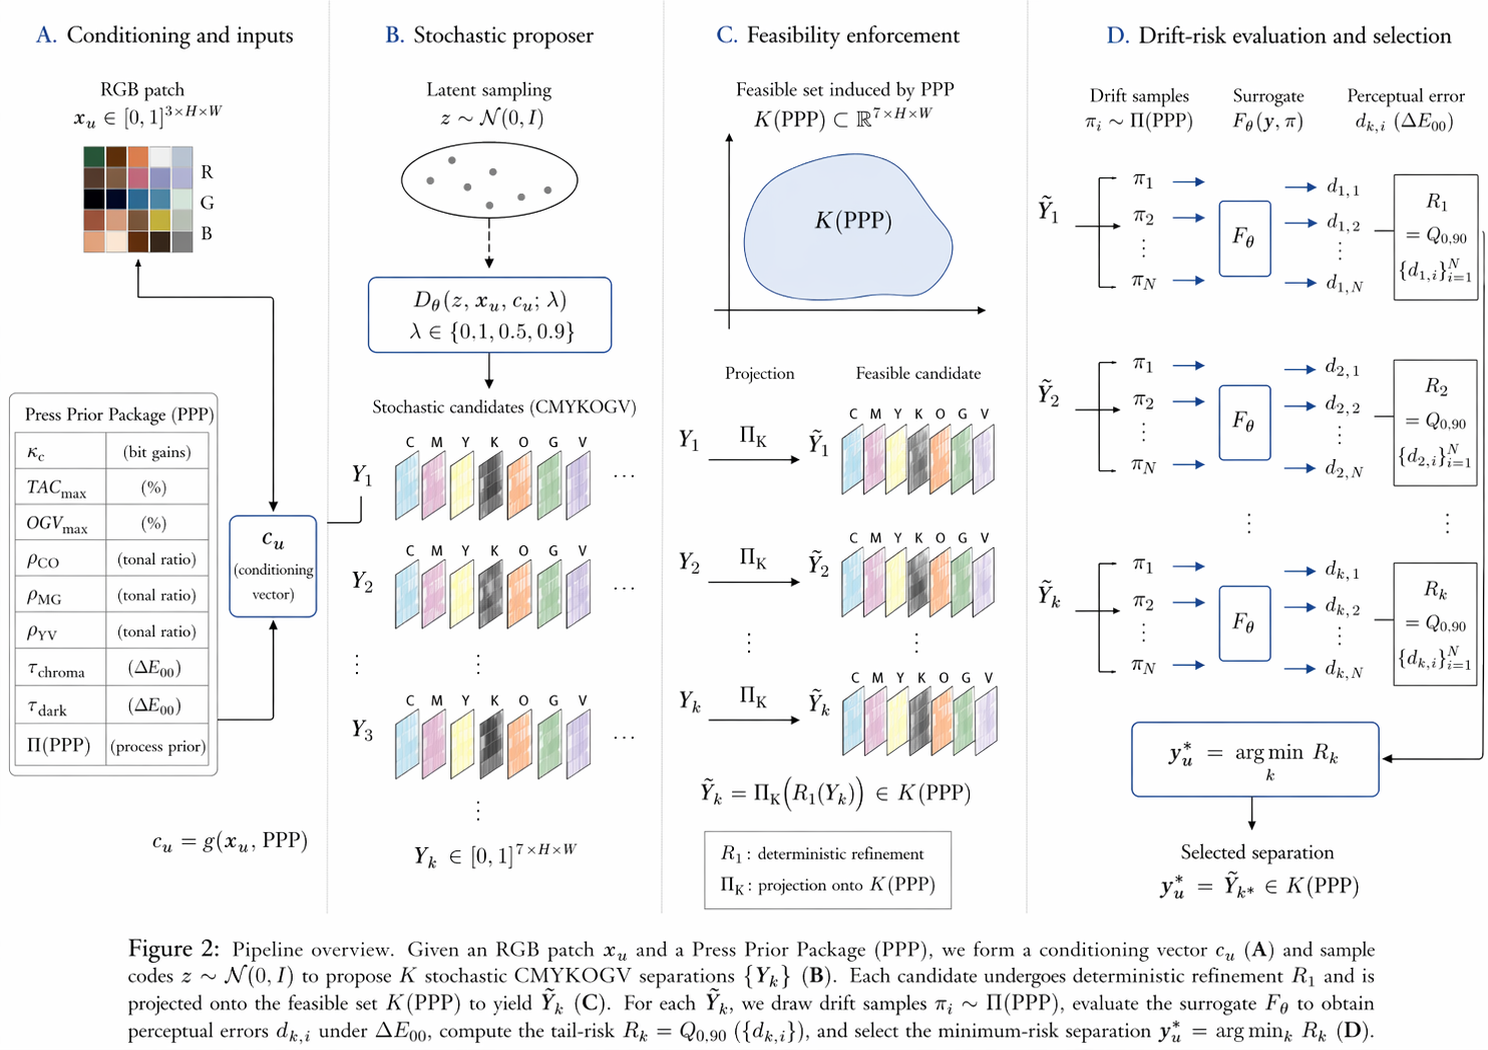
\includegraphics[width=\textwidth]{../figures/robustsep_system_manifold.png}
\caption{RobustSep operator-level pipeline.}
\label{fig:system_manifold}
\end{figure}

\subsection{Press Prior Package (PPP)}

A central design decision in RobustSep is that all press-specific knowledge is externalized into a structured inference-time object, the Press Prior Package, rather than baked into model weights. This allows a single trained model to be adapted across packaging process families by swapping the PPP, without re-training.

The PPP is a two-tier JSON object. The first tier is a base family token mapping to pre-calibrated ink constraints, drift parameters, and neutral detection thresholds for that process class. The second tier is a sparse override layer supplying job-specific values such as a measured TAC ceiling or a tighter per-channel cap; a binary override mask distinguishes fields that were deliberately set from those inherited from the family default. Five base families are currently defined depending upon their print characteristics. At inference time, the resolved PPP is encoded by a two-layer MLP into a 128-dimensional embedding $e_{\mathrm{PPP}} \in \mathbb{R}^{128}$. This is concatenated with a structure embedding $(\mathbb{R}^{32})$, an intent embedding $(\mathbb{R}^{128})$, and the scalar $\lambda$ to form the unified conditioning vector $c_u \in \mathbb{R}^{289}$, which drives Feature-wise Linear Modulation (FiLM) throughout both the CVAE proposer and the forward surrogate.

\begin{figure}[t]
\centering
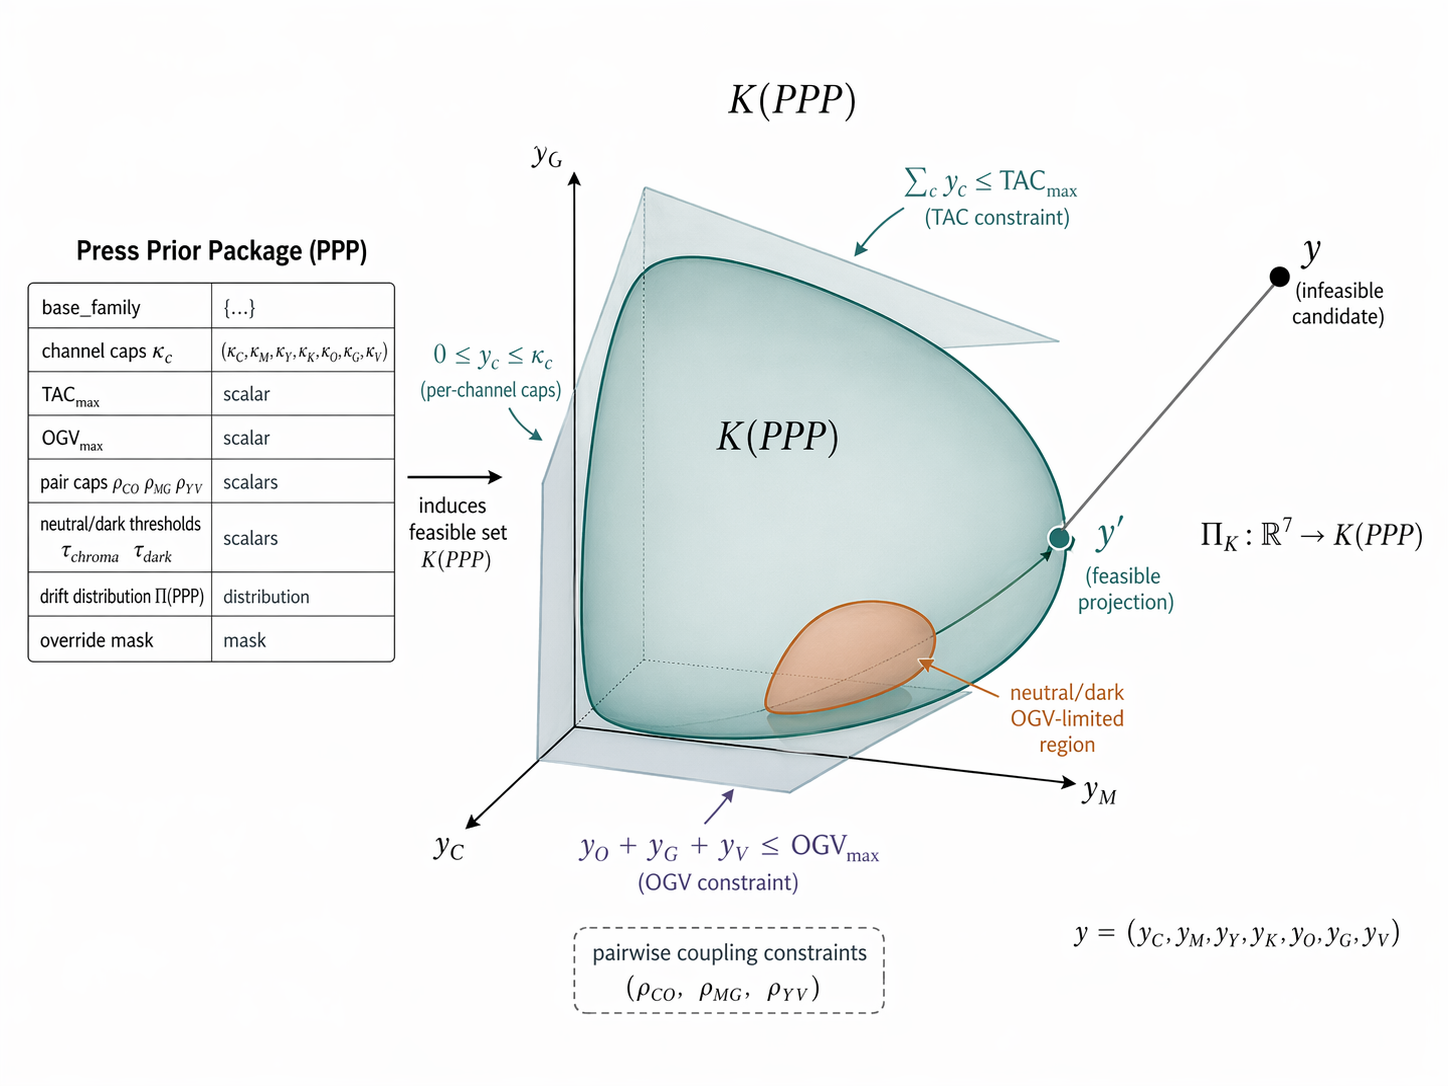
\includegraphics[width=\textwidth]{../figures/robustsep_ppp_feasibility.png}
\caption{The Press Prior Package induces the feasible set $K(\mathrm{PPP})$. Channel caps, TAC, OGV, pair-coupling, and neutral/dark constraints define a constrained envelope; $\Pi_K$ projects infeasible candidate separations back into this physically admissible region.}
\label{fig:ppp_feasibility}
\end{figure}

The PPP drift distribution $\Pi(\mathrm{PPP})$ models two dominant modes of press instability: per-channel ink-strength multipliers $m \in \mathbb{R}^7$ and monotone tone reproduction curve (TRC) perturbations. Drift is applied channel-wise as
\[
\pi(y)_c = \operatorname{clip}\!\bigl(\mathrm{TRC}_c(m_c \cdot y_c), 0, 1\bigr).
\]
Magnitude ranges are calibrated per process family such that gravure presses carry tighter tolerances than flexo, and OGV channels carry wider envelopes than CMYK because standardization of those inks is less mature. All drift sampling uses deterministic patch-level seeds to ensure exact reproducibility.

While this formulation captures variability in the printing process, it implicitly assumes that all perceptual deviations are equally consequential across the image, which is not the case in practice. Standard aggregate perceptual objectives weight all pixels uniformly, although a $\Delta E_{00}$ deviation on a brand-critical mark may be more consequential than the same deviation in a background gradient field. We address this by assigning each pixel to one of three intent classes, derived directly from the input RGB image through local statistics and edge analysis, with no learned components. The Brand class should be interpreted as a brand-critical or high-salience proxy unless external artwork annotations identify true brand marks. Flat pixels cover uniform or near-uniform fields where tonal stability and absence of banding matter most. Gradient pixels cover smooth tonal transitions like vignettes and continuous-tone imagery, where the primary failure mode is contouring rather than mean color error. Classification is resolved in strict priority order (Brand $>$ Gradient $>$ Flat), with unclassified pixels defaulting to Flat. Per-patch intent weights $(w_u^B, w_u^F, w_u^G)$ are the normalized pixel-class fractions for patch $u$. These enter the pipeline through two complementary paths: as constant per-pixel channels concatenated to the proposer's first-layer input (making intent spatially visible at the input level), and as a coarse $4\times 4$ intent raster processed through a dedicated intent embedding MLP. Both representations fold into $c_u$ and propagate via FiLM into every subsequent network block.

Having established a conditioning representation that encodes both spatial structure and perceptual priorities, the next step is to model the distribution of feasible ink separations under this conditioning.

\subsection{Proposer and Generation}

The proposer is a Conditional Variational Autoencoder (CVAE) \cite{kingma,sohn} that maps a $16\times 16$ RGB patch $x_u$, together with the conditioning vector $c_u \in \mathbb{R}^{289}$, to a distribution over plausible CMYKOGV ink patches. During training, the encoder $E_{\phi}$ maps the target patch and conditioning to a diagonal Gaussian posterior:
\[
(\mu, \log \sigma^2) = E_{\phi}(x_u, c_u), \qquad
q_{\phi}(z \mid x_u, c_u) = \mathcal{N}\!\bigl(z; \mu, \operatorname{diag}(\sigma^2)\bigr).
\]
A reparameterized latent sample
\[
z = \mu + \sigma \odot \varepsilon, \qquad \varepsilon \sim \mathcal{N}(0,I)
\]
is drawn and passed to the decoder. At inference, the encoder is unused; the decoder samples $z \sim \mathcal{N}(0,I)$ from the prior using a deterministic patch-level seed, generating
\[
Y_k = D_{\theta}(z, x_u, c_u) \in [0,1]^{7\times 16\times 16}.
\]

\begin{figure}[t]
\centering
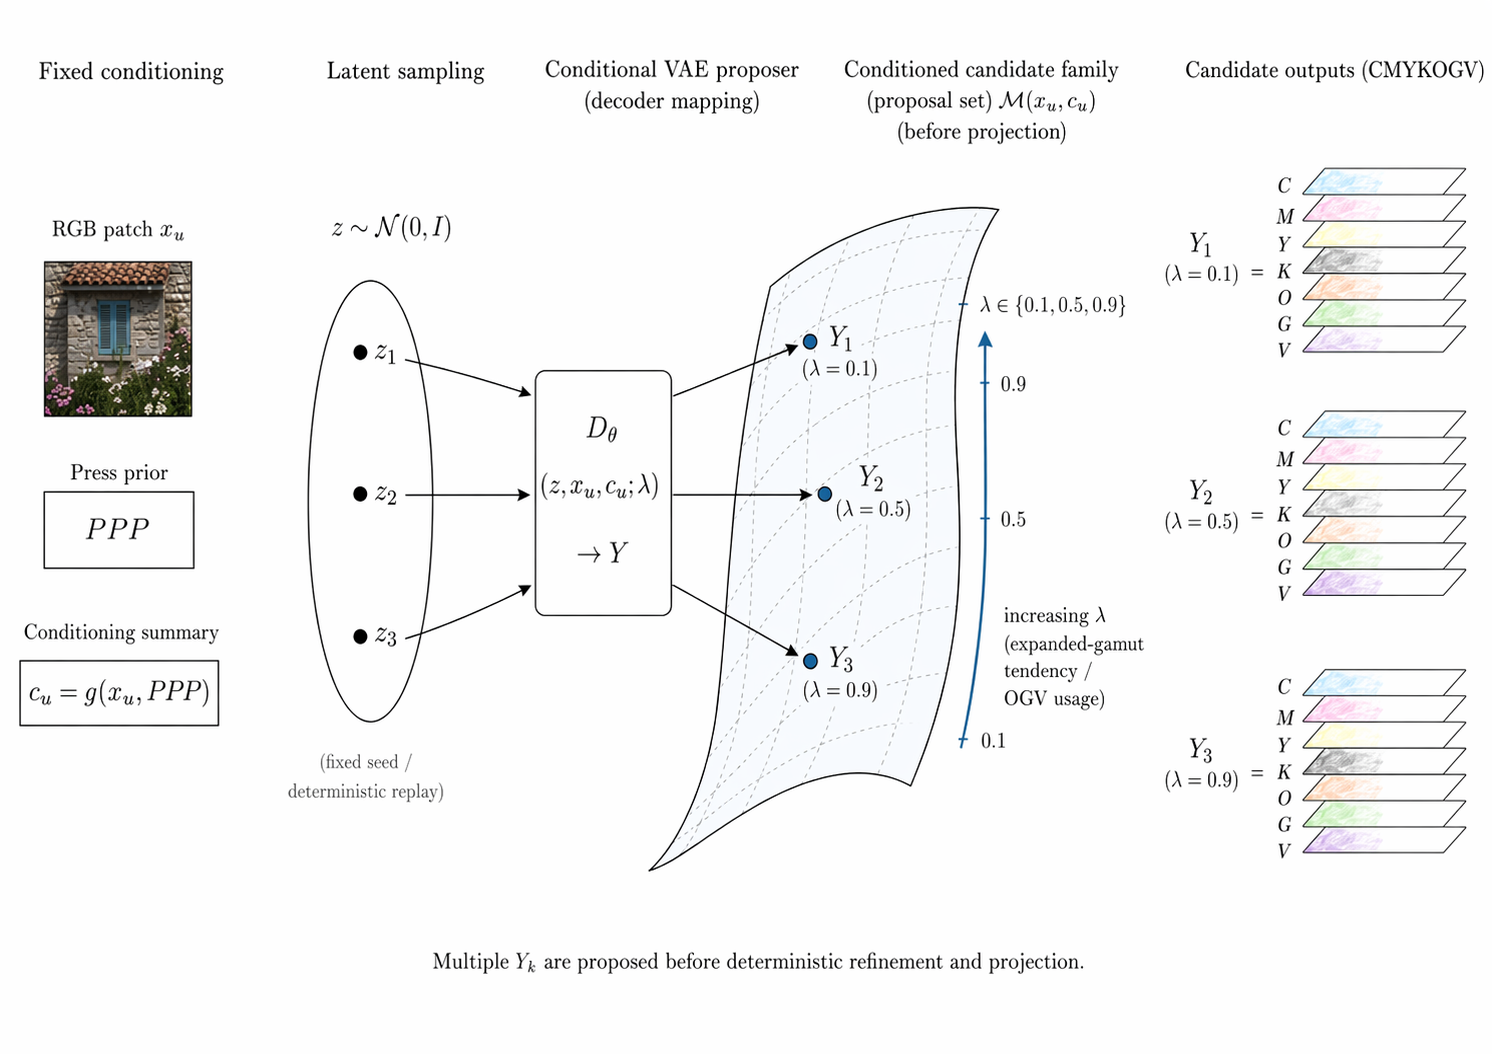
\includegraphics[width=\textwidth]{../figures/robustsep_proposer_manifold.png}
\caption*{\textbf{Conditioned stochastic proposal mechanism in RobustSep.} For a fixed RGB patch $x_u$ and conditioning vector $c_u$, the decoder $D_{\theta}$ maps latent samples $z \sim \mathcal{N}(0,I)$, together with $\lambda$, to a family of plausible CMYKOGV separations. Distinct latent samples yield alternative candidate separations $Y_k$, while $\lambda$ controls a structured axis of proposal variation prior to deterministic refinement and feasibility projection.}
\end{figure}

The encoder comprises five convolutional blocks E0--E4. E0 is a plain Conv$\rightarrow$GroupNorm$\rightarrow$SiLU block with no conditioning. E1 and E3 use strided convolutions (stride 2) to progressively reduce spatial resolution from $16\times 16$ to $4\times 4$; E2 and E4 are stride-1 refinement blocks. All of E1--E4 follow the pattern Conv$\rightarrow$GroupNorm$\rightarrow$FiLM$\rightarrow$SiLU. Global average pooling at $4\times 4$ produces a compact feature vector, projected by two linear heads to the latent mean $\mu$ and log-variance $\log \sigma^2$. The decoder D0--D5 reverses the hierarchy: D0 linearly projects $z$ to a $96\times 4\times 4$ tensor (no FiLM); D1--D5 are FiLM-conditioned Conv$\rightarrow$GroupNorm$\rightarrow$FiLM$\rightarrow$SiLU blocks with bilinear $2\times$ upsampling at D2 and D4, restoring $16\times 16$ resolution. A final $1\times 1$ sigmoid head produces the 7-channel output. FiLM scale is applied as $1 + \gamma_i$ to maintain near-identity initialization stability. Each FiLM-enabled block carries its own two-layer MLP head (Linear$\rightarrow$SiLU$\rightarrow$Linear) mapping $c_u$ to per-channel scale and shift vectors; heads are not shared across blocks.

The proposer is queried three times per patch, once per inference $\lambda$ value $\{0.1, 0.5, 0.9\}$, each with a distinct deterministic seed. A hinge penalty during training enforces that mean OGV ink usage is non-decreasing across these three $\lambda$ levels, so expanded-gamut ink usage scales predictably with the operator's intent. Separately, surrogate quality gates use a denser diagnostic probe schedule $\{0.0,0.3,0.6,0.9,1.0\}$ to evaluate candidate-ranking behavior; this probe schedule is not the default inference proposal schedule.

To support this controlled behavior, the proposer is trained with an objective that balances reconstruction fidelity, latent regularization, and perceptual alignment.

\paragraph{Proposer Loss.}

The CVAE proposer is trained with a three-term objective \cite{bo}:
\[
L_{\text{proposer}} = L^{\text{ink}}_{\text{recon}} + \beta(t) L_{\text{KL}} + \alpha_{\text{app}} L^{\text{ICC}}_{\text{app}}.
\]

The ink-space reconstruction term uses Smooth L1 (Huber) loss between the predicted patch $\hat{Y}$ and the synthetic CMYKOGV target $Y^*$:
\[
L^{\text{ink}}_{\text{recon}} =
\frac{1}{7HW}\sum_{c=1}^{7}\sum_{i,j}
\operatorname{SmoothL1}\!\bigl(\hat{Y}_{i,j,c}, Y^*_{i,j,c}\bigr).
\]

The KL divergence term regularizes the latent space toward the standard Normal prior:
\[
L_{\text{KL}} =
\frac{1}{2}\,\mathbb{E}\!\left[\mu^2 + \exp(\log \sigma^2) - \log \sigma^2 - 1\right]
\]
with a deterministic linear warm-up schedule
\[
\beta(t) = \beta_{\max}\min\!\left(1, \frac{t}{T_{\text{warmup}}}\right).
\]

The auxiliary appearance term encourages the predicted patch to match the ICC-rendered appearance of the target:
\[
L^{\text{ICC}}_{\text{app}} =
\frac{1}{3HW}\sum_{k=1}^{3}\sum_{i,j}
\operatorname{SmoothL1}\!\bigl(\hat{A}_{i,j,k}, A^*_{i,j,k}\bigr),
\]
where $\hat{A} = T_{\text{ICC}}(\hat{Y})$ and $A^* = T_{\text{ICC}}(Y^*)$ are the ICC-rendered Lab appearances of the predicted and target patches, respectively, under Relative Colorimetric intent with Black Point Compensation as defined in ICC color-management workflows \cite{icc}. The weight $\alpha_{\text{app}} \ll 1$ keeps this term a regularizer rather than a primary signal.

The forward surrogate is a lightweight Micro-CNN whose purpose is not artistic fidelity but computationally efficient, differentiable approximation of local ICC/proxy print-response changes for candidate ranking and robustness gating. Until measured seven-channel press characterization is available, the surrogate is treated as a local appearance-delta model rather than a global CMYKOGV-to-Lab renderer: it predicts $\Delta Lab$ around a stored reference $A^*$, and candidate appearance is reconstructed as $A^*+\widehat{\Delta Lab}$. This distinction is important because the current ICC/proxy teacher is anchor-calibrated rather than a measured absolute press model. The surrogate takes a $32\times 32$ CMYKOGV context window as input (providing spatial neighborhood context for halftone ink interactions and overprint effects), but is scored only on the inner $16\times 16$ region. It comprises eight convolutional blocks with channel progression $32 \rightarrow 32 \rightarrow 64 \rightarrow 64 \rightarrow 96 \rightarrow 96 \rightarrow 64 \rightarrow 32$. Block 0 is plain Conv$\rightarrow$GroupNorm$\rightarrow$SiLU with no FiLM; Blocks 1--7 follow Conv$\rightarrow$GroupNorm$\rightarrow$FiLM$\rightarrow$SiLU. Dilated convolutions (dilation rates 1, 2, 2, 4, 4, 1, 1 for Blocks 1--7) enlarge the effective receptive field without reducing spatial resolution. A $1\times 1$ linear head outputs the three-channel $\Delta Lab$ prediction.

To ensure that this surrogate remains faithful under both nominal and perturbed conditions, it is trained with symmetric supervision across drift states.

\paragraph{Surrogate Loss.}

The surrogate is trained under ICC/proxy teacher supervision rather than measured press Lab supervision. For each training example, the v2 shard schema stores a clean reference $A^*$, a nominal teacher target $L^{(n)}$, and a drifted teacher target $L^{(d)}$. The supervised targets are local deltas $\Delta L^{(n)}=L^{(n)}-A^*$ and $\Delta L^{(d)}=L^{(d)}-A^*$, not absolute Lab values. Both are supervised symmetrically using Huber loss with $\delta = 1.0$:
\[
L_{\text{nominal}} =
\frac{1}{HWC}\sum_{i,j,c}
\operatorname{Huber}_{\delta}\!\bigl(\widehat{\Delta L}^{(n)}_{i,j,c} - \Delta L^{(n)}_{i,j,c}\bigr),
\]
\[
L_{\text{drift}} =
\frac{1}{HWC}\sum_{i,j,c}
\operatorname{Huber}_{\delta}\!\bigl(\widehat{\Delta L}^{(d)}_{i,j,c} - \Delta L^{(d)}_{i,j,c}\bigr),
\]
\[
L_{\text{surrogate}} = L_{\text{nominal}} + L_{\text{drift}}.
\]

The symmetric equal-weighting prevents the surrogate from collapsing to a drift-invariant approximation, which would render robustness evaluation meaningless. The Huber loss is specifically chosen because extreme drift samples would otherwise dominate gradient updates. An epoch-level validation test monitors the ratio $L_{\text{drift}}/L_{\text{nominal}}$ within a stability band and flags sudden drift-loss collapse or persistent oscillation as training failures, ensuring the surrogate passes a quality gate before it is used in target generation.

To make drift effects explicit rather than implicit, the surrogate is additionally conditioned on the perturbation state itself. The FiLM conditioning vector is extended to $\mathbb{R}^{345}$ by appending a 56-dimensional drift embedding comprising per-channel ink-strength multipliers and monotone TRC perturbation parameters. This allows the model to learn structured interactions between specific perturbation profiles and their resulting appearance, rather than treating drift as unmodeled noise, thereby improving robustness evaluation fidelity across process families.

With a calibrated forward surrogate in place to reliably evaluate perceptual behavior under drift, the pipeline can shift from prediction to decision-making over candidate separations.

\subsection{Refinement and Assembly}

Every proposed candidate passes through a deterministic two-pass refiner before entering robustness evaluation. Pass 1 applies spatial regularity smoothing and neutral/dark stabilization to suppress high-frequency separation artifacts and ink-balance violations in perceptually sensitive regions. Pass 2 applies the feasibility projection operator $\Pi_K$, which enforces the full feasible set $K(\mathrm{PPP})$ by applying per-channel clipping, pair-cap enforcement, OGV limiting, neutral/dark OGV limiting, and TAC projection:
\[
Y'_c \leftarrow \operatorname{clip}(Y_c, 0, \kappa_c),
\]
\[
Y \leftarrow \operatorname{Proj}_{\sum_c Y_c \leq TAC_{\max}-\varepsilon}(Y').
\]
The small margin $\varepsilon$ prevents numerical instability at the exact TAC boundary. The TAC step is implemented as a capped-simplex downward projection over active CMYKOGV channels, not as unconstrained proportional rescaling. Projection is applied after every gradient step during target generation and unconditionally at inference, so the composed output
\[
\tilde{Y}_k = \Pi_K\bigl(R_1(Y_k)\bigr)
\]
is guaranteed to lie inside $K(\mathrm{PPP})$. Candidates requiring large projection corrections tend to accumulate higher robustness risk scores and are deprioritized during selection.

For each feasible candidate $\tilde{Y}_k$, $N = 32$ drift instances $\{\pi_i\}_{i=1}^{N}$ are sampled from $\Pi(\mathrm{PPP})$ using a deterministic patch-level seed. Drift is applied channel-wise within the $32\times 32$ context window:
\[
\tilde{Y}_{k,i} = \operatorname{clip}(\pi_i \odot \tilde{Y}_k, 0, 1).
\]
The surrogate predicts local CIELab appearance deltas, which are added to the reference appearance for scoring:
\[
\widehat{LAB}_{k,i} = A_u^* + F_{\theta}(\tilde{Y}_{k,i}, c_u)
\]
for each drifted candidate. Perceptual error is aggregated using per-patch intent weights:
\[
d_{k,i} =
\sum_{r \in \{B,F,G\}} w_r \cdot \frac{1}{|P_r|}
\sum_{(i,j)\in P_r}
\Delta E_{00}\!\bigl(\widehat{LAB}_{k,i,j}, A^*_{u,i,j}\bigr),
\]
where $P_r$ is the set of pixels belonging to intent class $r$ within the patch. The robustness risk score is
\[
R_k = Q_{0.90}\bigl(\{d_{k,i}\}_{i=1}^{N}\bigr).
\]
For a finite set $S$, the empirical quantile is defined deterministically as
\[
Q_q(S) = \operatorname{sort}(S)_{\lceil q|S| \rceil - 1},
\]
using zero-based indexing after sorting in ascending order.

Figure~\ref{fig:drift_risk_selection} visualizes the candidate-wise drift evaluation and quantile-based selection rule.

\begin{figure}[t]
\centering
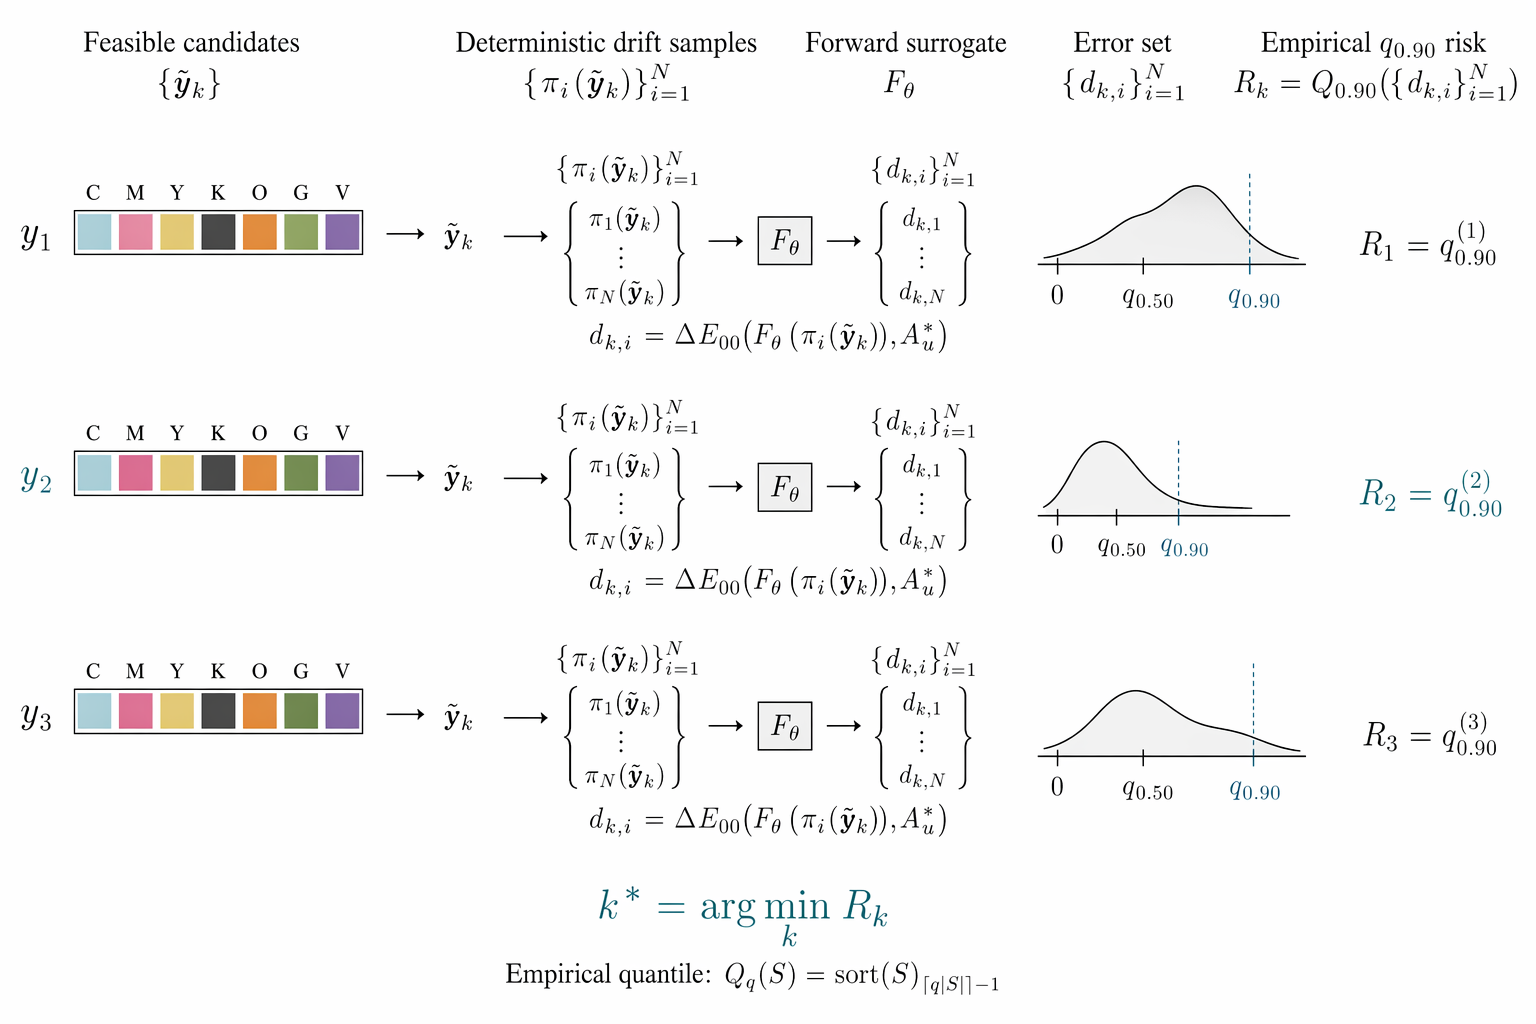
\includegraphics[width=\textwidth]{../figures/robustsep_drift_risk_selection.png}
\caption{Drift-risk candidate selection. Each feasible CMYKOGV candidate is evaluated across deterministic PPP-conditioned drift samples; RobustSep selects the candidate with the lowest 90th-percentile $\Delta E_{00}$ risk rather than the lowest nominal or mean error.}
\label{fig:drift_risk_selection}
\end{figure}

The minimum-risk feasible candidate is selected; ties are broken by nominal error computed under identity drift. Per-pixel ink usage statistics, TAC margin, neutral/dark stability flags, and a spatial regularity score are also logged at this stage for audit purposes.

If no candidate survives the robustness gate, an escalation policy first increases $K$ up to a maximum of 5, regenerating proposals with independent latent samples and repeating refinement and drift evaluation. Only if this coverage escalation also fails is the drift sample count raised as a secondary measure. All escalation events are recorded in the decision report $R$, with additional budget optionally allocated to patches carrying high brand or gradient content.

After per-patch processing, the full-resolution CMYKOGV image is assembled from overlapping $16\times 16$ patches extracted with stride $t < 16$. Each pixel $(i,j)$ receives a weighted blend over all contributing patches $\Omega(i,j)$:
\[
\hat{C}_{\text{image}}(i,j)
=
\sum_{u \in \Omega(i,j)}
w_u(i,j)\cdot \tilde{Y}_u^*(i-u_x, j-u_y),
\qquad
\sum_u w_u(i,j) = 1.
\]
Blending weights are tapered smoothly toward patch boundaries (suppressing blocking artifacts) and sharpened for edge-classified patches (preserving spatial sharpness of separation boundaries). A final global feasibility pass applies $\Pi_K$ to the assembled image to correct any TAC violations introduced at patch overlap zones. A decision report $R$ is emitted alongside the output, recording the PPP configuration, constraint tightness indicators, risk score distributions, escalation events, and fallback activations, to support downstream audit and iterative PPP refinement.

\section{Evaluation}

\subsection{Datasets and Splits}

\begin{sloppypar}
We evaluate the proposed RobustSep pipeline on staged patch manifests spanning three source families: RobustSep raster/vector patches, DocLayNet layout patches, and SKU-110K product/packaging imagery. The current v1.1 split manifests contain 460,969 train patches, 57,344 validation patches, and 24,576 test patches; surrogate training shards contain two drift-conditioned examples per patch, yielding 921,938 train, 114,688 validation, and 49,152 test examples. Current shards use the \texttt{ones} alpha policy because transparent regions were filtered before shard generation.
\end{sloppypar}

\begin{table}[htbp]
\centering
\caption{Evaluation Split Composition}
\label{tab:dataset_splits}
\begin{tabular}{lrrr}
\toprule
Source family & Train patches & Val patches & Test patches \\
\midrule
RobustSep & 165,505 & 20,480 & 8,192 \\
DocLayNet & 136,328 & 16,384 & 8,192 \\
SKU-110K & 159,136 & 20,480 & 8,192 \\
\midrule
Total patches & 460,969 & 57,344 & 24,576 \\
Surrogate examples & 921,938 & 114,688 & 49,152 \\
\bottomrule
\end{tabular}
\end{table}

\subsection{Baselines}

We compare RobustSep against four operational baselines. The ICC CMYK baseline uses the staged ICC separation without OGV expansion. The projected ICC baseline embeds ICC CMYK into CMYKOGV with OGV initialized to zero and applies $\Pi_K$. A learned deterministic baseline is included when an unconstrained RGB-to-ink model checkpoint is available. Component ablations remove the deterministic refiner, the forward surrogate ranking stage, or the PPP feasibility constraints.

\subsection{Protocol}

All experiments use $16\times16$ scored patches and $32\times32$ CMYKOGV context windows. Unless otherwise stated, robustness evaluation draws $N=32$ deterministic drift samples from $\Pi(\mathrm{PPP})$ and reports finite-quantile tail risk using $Q_q(S)=\operatorname{sort}(S)_{\lceil q|S|\rceil-1}$. The default PPP base family is \texttt{film\_generic\_conservative}, with any job-specific overrides recorded in the canonical PPP JSON. All stochastic components are replayable from the root seed, source identifier, patch coordinate, PPP hash, and stage name. Split manifests, target records, surrogate shards, checkpoints, and evaluation reports are hash-linked so reported numbers can be traced to the exact artifacts used to compute them.

\subsection{Primary Metrics}

We adopt a comprehensive set of metrics inspired by prior works such as Chen et al.\ and Zeng et al.\ to ensure a rigorous comparison, but prioritize metrics that directly test robust print feasibility.

\begin{itemize}
    \item \textbf{Drift-Robust Color Fidelity:} Primary metrics are mean, median, 75th-, 90th-, and 95th-percentile CIE $\Delta E_{00}$ under PPP-sampled drift, together with the percentage of patches exceeding operational $\Delta E_{00}$ thresholds.
    \item \textbf{Print Feasibility:} Quantified via TAC violation rate, per-channel cap violations, OGV-cap violations, neutral/dark OGV violations, pair-cap violations, ink consumption per channel, Neutral Gray Balance stability, and K-channel distribution statistics (mean, std).
    \item \textbf{Decision Quality and Runtime:} Reported using surrogate candidate-ranking Spearman correlation, top-1 agreement with the teacher/proxy ranking, teacher-risk regret for the surrogate-selected candidate, escalation rate, fallback rate, and runtime per patch or megapixel.
\end{itemize}

\subsection{Secondary Metrics}

Secondary diagnostics include MSE, PSNR, and SSIM in Lab or luminance space; Edge Error (\%) for fine text and border preservation; and qualitative panels comparing RGB target appearance, rendered separation appearance, and $\Delta E_{00}$ error maps. These metrics are reported for interpretability but do not replace the drift-risk and feasibility metrics above.

\subsection{Quantitative Results}

The quantitative performance of RobustSep compared to standard baseline approaches is presented in Table~\ref{tab:quant_results}. Furthermore, Table~\ref{tab:percentile_robustness} details the robustness characteristics at the 50th, 75th, 90th, and 95th percentiles to demonstrate the system's resilience to tail-risk drift events.

\begin{table}[htbp]
\centering
\caption{Quantitative Performance Comparison}
\label{tab:quant_results}
\begin{tabular}{p{0.34\textwidth}p{0.56\textwidth}}
\toprule
Metric & Reported statistic \\
\midrule
Mean $\Delta E_{00}$ under drift & Mean over held-out test patches \\
Median $\Delta E_{00}$ under drift & 50th percentile over held-out test patches \\
Q90 $\Delta E_{00}$ under drift & 90th percentile drift-risk statistic \\
Q95 $\Delta E_{00}$ under drift & 95th percentile drift-risk statistic \\
$\Delta E_{00}$ threshold exceedance & Percent above operational threshold \\
MSE / PSNR / SSIM & Secondary Lab/luminance similarity diagnostics \\
Edge Error & Percent edge disagreement \\
TAC violation rate & Percent pixels or patches exceeding $TAC_{\max}$ \\
Channel-cap violations & Count by CMYKOGV channel \\
OGV/neutral/pair violations & Count by feasibility constraint type \\
Ink Usage & Mean channel coverage by ink \\
Gray Balance & Neutral/dark chroma deviation \\
K Mean / K Std & Black-channel distribution statistics \\
Spearman candidate ranking & Candidate-risk ordering correlation \\
Top-1 candidate agreement & Agreement with teacher/proxy best candidate \\
Teacher-risk regret & Risk gap between surrogate-selected and teacher-best candidate \\
Escalation / fallback rate & Percent patches requiring escalation or fallback \\
Runtime per patch & Mean wall-clock processing time \\
\bottomrule
\end{tabular}
\end{table}

\begin{table}[htbp]
\centering
\caption{Percentile Analysis (Robustness)}
\label{tab:percentile_robustness}
\begin{tabular}{lcccc}
\toprule
Metric & 50th & 75th & 90th & 95th \\
\midrule
$\Delta E_{00}$ & reported & reported & reported & reported \\
Edge Error & reported & reported & reported & reported \\
TAC & reported & reported & reported & reported \\
\bottomrule
\end{tabular}
\end{table}

\subsection{Visual Results}

Qualitative visual comparisons highlighting process drift robustness are provided in Figure~\ref{fig:visual_comparison}. The layout provides a direct juxtaposition of the original target and our separation output.

\begin{figure}[htbp]
\centering
\fbox{\parbox{0.8\textwidth}{\vspace{2em}\centering Evaluation image grid generated from held-out visual examples\\Layout: Original RGB $\mid$ Rendered Separation $\mid$ $\Delta E_{00}$ Error Map\vspace{2em}}}
\caption{Qualitative Comparison of Separation Outcomes}
\label{fig:visual_comparison}
\end{figure}

\subsection{Distribution Analysis}

To better understand the variance and tail events produced under print drift, we analyze the distribution of key separation metrics across our entire test set.

\begin{figure}[htbp]
\centering
\fbox{\parbox{0.65\textwidth}{\vspace{2em}\centering $\Delta E_{00}$ histogram generated from evaluation report\vspace{2em}}}
\caption{$\Delta E_{00}$ perceptual error distribution. The right tail characterizes worst-case behavior under PPP-sampled drift.}
\label{fig:de_dist}
\end{figure}

\begin{figure}[htbp]
\centering
\fbox{\parbox{0.65\textwidth}{\vspace{2em}\centering TAC histogram generated from evaluation report\vspace{2em}}}
\caption{TAC distribution across the evaluation dataset, including the fraction exceeding the PPP threshold.}
\label{fig:tac_dist}
\end{figure}

\begin{figure}[htbp]
\centering
\fbox{\parbox{0.65\textwidth}{\vspace{2em}\centering K-channel histogram or KDE generated from evaluation report\vspace{2em}}}
\caption{K-Channel (Black Ink) Usage Distribution across Separation Candidates.}
\label{fig:k_dist}
\end{figure}

\subsection{Ablation and Failure Analysis}

We perform an ablation study to isolate the impact of our core architectural components: the deterministic refiner, the forward surrogate, and the PPP constraints. The results are summarized in Table~\ref{tab:ablation}. Failure analysis additionally reports cases where the system is expected to be most stressed: saturated neon colors near the expanded-gamut boundary, dark neutrals where OGV must be suppressed, thin text or borders, high OGV constraint pressure, and severe drift samples.

\begin{table}[htbp]
\centering
\caption{Ablation Study Results}
\label{tab:ablation}
\begin{tabular}{lccc}
\toprule
Variant & Drift $\Delta E_{00}$ & Feasibility & Edge Error \\
\midrule
Full Model & reported & reported & reported \\
w/o Refiner & reported & reported & reported \\
w/o Surrogate & reported & reported & reported \\
w/o PPP Constraints & reported & reported & reported \\
\bottomrule
\end{tabular}
\end{table}

\subsection{Discussion}

The comprehensive evaluations are designed to separate nominal color fidelity from the stronger requirements of robust print feasibility. RobustSep should be judged primarily by drift-tail $\Delta E_{00}$, feasibility violations, candidate-ranking agreement, and escalation behavior, with secondary visual metrics used to interpret failure modes rather than to replace the print-specific criteria.

\begin{thebibliography}{11}

\bibitem{ulichney}
R. Ulichney,
\textit{Digital Halftoning}.
Cambridge, MA, USA: MIT Press, 1987.

\bibitem{rodriguez}
M. Rodriguez,
``A graphic arts perspective on RGB-to-CMYK conversion,''
in \textit{Proc. IEEE Int. Conf. Image Processing (ICIP)}, Washington, DC, USA, 1995, pp. 319--322.
doi: 10.1109/ICIP.1995.537479.

\bibitem{zeng}
H. Zeng,
``3D color separation maximizing the printer gamut,''
in \textit{Proc. SPIE 5008, Color Imaging VIII}, Jan. 2003.
doi: 10.1117/12.472012.

\bibitem{marcu}
G. Marcu and K. Iwata,
``RGB-CMYK color conversion by application of the neural networks,''
in \textit{IS\&T/SID Color Imaging Conf.}, 1993, pp. 27--32.

\bibitem{chen}
Z. Chen, Z. Wang, B. Sheng, C. Li, R. Shen, and P. Li,
``Dynamic RGB-to-CMYK conversion using visual contrast optimisation,''
\textit{IET Image Process.}, vol. 11, no. 7, pp. 539--549, 2017.
doi: 10.1049/iet-ipr.2016.0400.

\bibitem{bo}
M. Bo and P. Cao,
``Color space transformation model based on the residual attention mechanism,''
in \textit{Proc. ACM ICVIP}, 2025, pp. 492--499.
doi: 10.1145/3730436.3730518.

\bibitem{icc}
International Color Consortium,
\textit{ICC.1:2010 --- Image Technology Colour Management: Architecture, Profile Format and Data Structure},
2010.

\bibitem{kingma}
D. P. Kingma and M. Welling,
``Auto-encoding variational Bayes,''
in \textit{Proc. ICLR}, 2014.

\bibitem{sohn}
K. Sohn, H. Lee, and X. Yan,
``Learning structured output representation using deep conditional generative models,''
in \textit{Proc. NeurIPS}, 2015.

\bibitem{luo}
M. R. Luo, G. Cui, and B. Rigg,
``The development of the CIE 2000 colour-difference formula: CIEDE2000,''
\textit{Color Res. Appl.}, vol. 26, no. 5, pp. 340--350, 2001.
doi: 10.1002/col.1049.

\bibitem{kipphan}
H. Kipphan, Ed.,
\textit{Handbook of Print Media}.
Berlin, Germany: Springer, 2001.

\end{thebibliography}

\end{document}
